\documentclass[aps,prb,twocolumn,superscriptaddress,longbibliography,floatfix]{revtex4-2}
\usepackage{amsmath,amssymb,bm}
\usepackage{graphicx}
\usepackage{dcolumn}
\usepackage[colorlinks=true,linkcolor=blue,citecolor=blue,urlcolor=blue]{hyperref}

\newcommand{\vS}{\mathbf S}
\newcommand{\vh}{\mathbf h}
\newcommand{\vu}{\mathbf u}
\newcommand{\vv}{\mathbf v}
\newcommand{\vr}{\mathbf r}
\newcommand{\ueff}{u_{\rm eff}}
\newcommand{\vueff}{\mathbf u_{\rm eff}}
\newcommand{\kT}{k_BT}
\newcommand{\Beff}{B_{\rm eff}}
\newcommand{\dd}{\mathrm d}
\newcommand{\avg}[1]{\langle #1\rangle}

\begin{document}

\title{Precession as a hidden field: vorticity-selected topological charge and\\ thermal skyrmion statistics under nonreciprocal spin couplings}

\author{Changyeon Won}
\email{cywon@khu.ac.kr}
\affiliation{Department of Physics, Kyung Hee University, Seoul 02447, Republic of Korea}

\date{\today}

\begin{abstract}
In thermal equilibrium a two-dimensional magnet acquires a net topological charge only when a magnetic field and spin--orbit coupling act together. We show that this rule changes qualitatively when the magnet is driven by nonreciprocal spin couplings, which arise whenever a spin current or another dissipative flow is integrated out. Because an improper spin rotation reverses the precessional term of the Landau--Lifshitz equation but not the damping, precession itself plays the role of the field. A net charge then requires only that every operation reversing the orientation of the plane be broken. A uniform current therefore cannot create net charge at any order; the vorticity of the flow can, and an out-of-plane spin-torque polarization combined with interfacial Dzyaloshinskii--Moriya interaction acts as an effective field $\Beff=-(11/72)\,\delta D_z/\alpha$. At high temperature the topological density couples locally to vorticity with strength $\kappa(T)=\kappa_0[1+(8/9)J/\kT]$. At low temperature the skyrmion Hall drift is an exact gradient flow in the stream function of the effective drift $\ueff=(\beta-\alpha)u/\alpha$, which fixes a Boltzmann law for skyrmion positions, a drive-independent density of free skyrmions, and a pair correlation shadowed upstream of the Hall separation. Finally, we identify a second, previously overlooked channel: even at $\beta=\alpha$ the local rotation of a sheared current acts on the spins as a precession-only field, which in the weak-damping regime is equivalent to a Zeeman field $\Beff=-\omega/2$. Large-scale stochastic simulations of a chiral ferromagnet confirm this channel---odd in the rotation, local, independent of damping, and following the predicted dependence on temperature and DMI strength to within $15\pm8\%$. All other analytic predictions agree with simulations without fitting parameters.
\end{abstract}

\maketitle

%=====================================================================
\section{Introduction}
%=====================================================================

Magnetic skyrmions, merons and vortices are two-dimensional textures that carry a topological charge
\begin{equation}
Q=\frac{1}{4\pi}\int \mathbf n\cdot(\partial_x\mathbf n\times\partial_y\mathbf n)\,\dd^2r .
\label{eq:Q}
\end{equation}
They have become central objects of spintronics because the charge makes them robust, mobile and countable~\cite{BelavinPolyakov1975,Muhlbauer2009,NagaosaTokura2013,Fert2017}. Which sign of $Q$ a magnet prefers is fixed by symmetry. In thermal equilibrium the Boltzmann weight is even under $Q\to-Q$ unless two symmetries are broken together: a magnetic field must break time reversal and fix the core polarity, and spin--orbit coupling, through the Dzyaloshinskii--Moriya interaction (DMI), must break the mirrors and fix the winding. Without either, thermally excited skyrmions and antiskyrmions appear in equal numbers.

Current-driven magnets are not in equilibrium, and the effective couplings between their spins need not be reciprocal. Integrating out a flowing, dissipative medium---conduction electrons carrying a spin current, or magnons driven by a temperature gradient---produces exchange couplings whose transpose symmetry is broken, $J_{ij}\neq J_{ji}$. Spin-transfer and spin--orbit torques are the familiar examples~\cite{ZhangLi2004,Thiaville2005}. Nonreciprocal interactions have recently been shown to generate new phases and new dynamical states in active and driven matter~\cite{Fruchart2021,Hanai2024,Das2002}, but their consequences for topological textures have not been organized.

In this paper we ask a sharp question: \emph{when can a nonreciprocal coupling create a net topological charge, and how do topological defects move, pair and nucleate under it?} The answer has four layers, and each layer contains a result that we believe is new.

\emph{(i) Symmetry.} An improper spin rotation reverses the precessional term of the Landau--Lifshitz (LL) equation but leaves the damping intact. Out of equilibrium, precession therefore already breaks the symmetry that a magnetic field breaks in equilibrium. The only remaining requirement for $\avg{Q}\neq0$ is that no operation reversing the orientation of the plane survives [Fig.~\ref{fig:concept}]. This gives exact selection rules, valid to all orders and at all temperatures (Sec.~\ref{sec:symmetry}). A uniform current never produces net charge in a mirror-symmetric film; circulation of the current does.

\emph{(ii) High temperature.} The topological density couples locally to the vorticity of the drive, with a coefficient we compute to second order. An out-of-plane spin-torque polarization acts as a magnetic field on the topological charge, $\Beff=-(11/72)\delta D_z/\alpha$ (Sec.~\ref{sec:highT}).

\emph{(iii) Low temperature.} For well-formed skyrmions, the charge-odd part of the Thiele motion---the skyrmion Hall drift---is an exact gradient flow in the stream function of the drive. Positions obey a Boltzmann law; free skyrmion--antiskyrmion pairs escape with a probability we obtain in closed form, their density is independent of the drive, and their correlation is shadowed \emph{upstream}, opposite to naive expectation (Secs.~\ref{sec:lowT} and~\ref{sec:pairs}).

\emph{(iv) Nucleation.} Symmetry permits a nucleation bias proportional to vorticity. Simulations of a chiral ferromagnet show that this bias does not vanish at $\beta=\alpha$, where all effects carried by the effective drift disappear. We trace the residual to the local rotation of the sheared current, which acts on the spins as a precession-only field and, in the weak-damping regime relevant to experiment, as a Zeeman field $\Beff=-\omega/2$ (Sec.~\ref{sec:nucleation}).

A recurring theme is that the drive acts on topological statistics through the combination
\begin{equation}
\ueff=\frac{\beta-\alpha}{\alpha}\,u ,
\label{eq:ueff}
\end{equation}
which vanishes when the nonadiabatic parameter $\beta$ equals the damping $\alpha$. This invariant also sets the effective spin-wave DMI and the Walker threshold of domain walls in a companion study~\cite{Companion}. The rotational channel of item (iv) is the one exception, and its existence is a central finding of this work. Throughout we confirm analytic predictions with stochastic LL simulations and Thiele-level particle simulations, without fitting parameters except where stated.

%=====================================================================
\section{Model}\label{sec:model}
%=====================================================================

We consider classical unit spins $\vS_i$ on a square lattice (spacing $a=1$) with a reciprocal energy $E$ and a nonreciprocal field-like coupling. The stochastic LL equation reads
\begin{align}
\dd\vS_i={}&\Big[-c_p\,\vS_i\times\big(\vh_i+\vh_i^{N}\big)-\alpha\,\vS_i\times(\vS_i\times\vh_i)\Big]\dd t\nonumber\\
&-\sqrt{2\alpha\kT}\;\vS_i\times\circ\,\dd\mathbf W_i ,
\label{eq:LL}
\end{align}
with $\vh_i=-\partial E/\partial\vS_i$ and Stratonovich noise. The sign $c_p=\pm1$ of the gyromagnetic ratio is kept explicit for the symmetry argument; $\alpha$ is the LL damping. For $\vh^N=0$ the stationary measure is $e^{-E/\kT}$ for either sign of $c_p$.

\emph{Nonreciprocal coupling.} The field-like (FL) nonreciprocal field is $\vh^N_i=\sum_jN_{ij}\vS_j$ with $N_{ji}=-N_{ij}^{T}$. Its scalar part is a directed exchange bias $\delta J_{ij}=-\delta J_{ji}$. For a flow with local unit direction $\hat{\vv}(\vr)$,
\begin{equation}
\delta J_{ij}=\delta J\,\big(\hat e_{ij}\cdot\hat{\vv}(\vr_{ij})\big),\qquad \omega=\hat z\cdot\nabla\times\hat{\vv},
\label{eq:dJ}
\end{equation}
where $\hat e_{ij}$ is the bond direction and $\omega$ the vorticity. Its vector part is an exchange-even rotation, $N_{ij}=N_{ji}=\delta D\,[\mathbf n]_\times$. With spin--orbit coupling (SOC) $\mathbf n$ is locked to the lattice; without it $\mathbf n$ lives in spin space only.

\emph{Current-driven realization.} The adiabatic and nonadiabatic Zhang--Li torques~\cite{ZhangLi2004,Thiaville2005}, $-(\vu\cdot\nabla)\vS+\beta\vS\times(\vu\cdot\nabla)\vS$, are a damping-like and a field-like bias of this form. In the frame comoving with domain walls and skyrmions, the field-like component that survives is proportional to $\ueff$ of Eq.~\eqref{eq:ueff}.

\emph{Thiele level.} A rigid skyrmion with gyrocoupling $G=4\pi Qs$ ($s$ is the spin density) and dissipation dyadic $\mathcal D$ obeys~\cite{Thiele1973}
\begin{equation}
G\,\hat z\times(\vv-\vu)+\mathcal D\,(\alpha\vv-\beta\vu)=\mathbf F+\bm\xi,
\label{eq:thiele}
\end{equation}
with $\avg{\xi_a(t)\xi_b(t')}=2\alpha\mathcal D\kT\,\delta_{ab}\delta(t-t')$.

\emph{Lattice charge.} The corner-chirality charge $Q_\chi=(8\pi)^{-1}\sum\chi$ sums $\chi_{\rm UR}=\vS_i\cdot(\vS_{i+\hat x}\times\vS_{i+\hat y})$ and its three rotations over all sites. It is odd under every lattice mirror for each configuration separately. The Berg--L\"uscher charge~\cite{BergLuscher1981}, built from solid angles of a fixed triangulation, is integer valued and is used to count nucleation events.

%=====================================================================
\section{Topological-charge selection rules}\label{sec:symmetry}
%=====================================================================

\begin{figure*}[t]
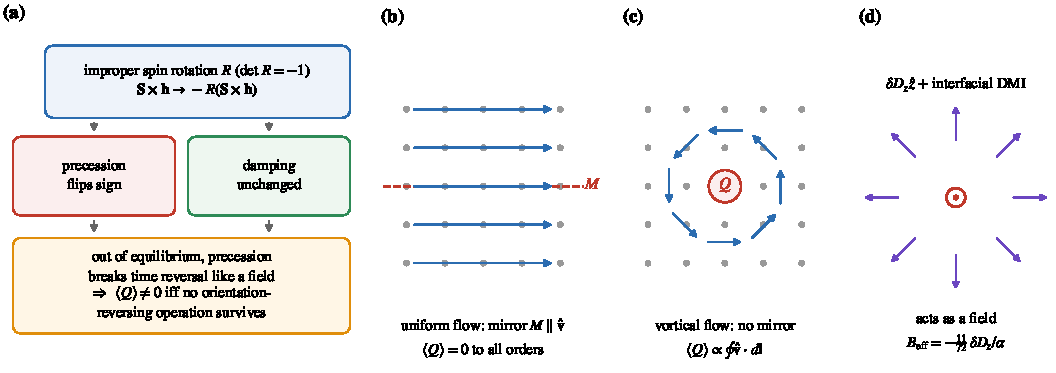
\includegraphics[width=\textwidth]{figs/concept.pdf}
\caption{Why precession acts as a field out of equilibrium. (a)~Under an improper spin rotation $R$ the precessional term of Eq.~\eqref{eq:LL}, which contains one cross product, changes sign, while the damping term, which contains two, does not. In equilibrium the stationary measure does not depend on the sign of precession; out of equilibrium it does, so precession breaks time reversal just as a field does. The only remaining condition for $\avg{Q}\neq0$ is the absence of orientation-reversing operations. (b)~A uniform flow leaves the mirror that contains it, and $\avg{Q}=0$ exactly. (c)~A vortical flow leaves no mirror, and the net charge is proportional to the circulation. (d)~With interfacial DMI, an out-of-plane bias $\delta D_z\hat z$ acts on the topological charge as a magnetic field.}
\label{fig:concept}
\end{figure*}

The topological density contains two spatial derivatives and a triple product of spins. Under an operation $g$ that acts on the plane with orientation sign $\epsilon_s$ ($-1$ for mirrors and in-plane twofold axes) and on spin space with an O(3) matrix $R$,
\begin{equation}
Q\;\to\;\epsilon_s\,\det R\;Q .
\label{eq:Qtrans}
\end{equation}

\emph{Theorem 1 (equivariance).} Let $g=(\pi,R)$ act as $\vS_i\to R\,\vS_{\pi^{-1}(i)}$, with $\pi$ a lattice isometry and $R\in{\rm O}(3)$. Then $g$ maps the model of Eq.~\eqref{eq:LL} with precession sign $c_p$ and couplings $\mathcal C$ onto the model with $\det R\cdot c_p$ and $g\cdot\mathcal C$. Because the noise is elliptic on $(S^2)^N$, the stationary distribution is unique and transforms accordingly.

\emph{Proof.} For any $R\in{\rm O}(3)$, $Ra\times Rb=(\det R)\,R(a\times b)$. The precession term contains one cross product and acquires $\det R$; the damping term contains two and is invariant. The FL nonreciprocal field enters only through the precession. The noise term flips sign at most, which $\dd\mathbf W\to-\dd\mathbf W$ absorbs. $\square$

\emph{Theorem 2 (selection rule).} If the couplings are invariant under $g$, then
\begin{equation}
\avg{Q}_{c_p}=\epsilon_s\,\det R\;\avg{Q}_{\det R\cdot c_p}.
\label{eq:selection}
\end{equation}
Three consequences follow. First, if an operation with $R=\mathbb 1$ and $\epsilon_s=-1$ leaves the couplings invariant, then $\avg{Q}=0$ and $P(Q)=P(-Q)$ at every temperature and to all orders in the drive. Second, in equilibrium the measure is independent of $c_p$; a bilinear $E$ is invariant under $R=-\mathbb 1$, so $\avg{Q}_{\rm eq}=0$ without a field. Third, out of equilibrium $\avg{Q}$ is odd in the overall sign of precession. Precession thus supplies the time-reversal breaking that a field supplies in equilibrium [Fig.~\ref{fig:concept}(a)].

\emph{Without SOC} spatial operations move sites but leave spins untouched ($R=\mathbb 1$). A uniform polar bias $\delta J_{ij}=\delta J\,\hat e_{ij}\cdot\hat{\vv}$ leaves the mirror that contains $\hat{\vv}$, so $\avg{Q}=0$ exactly when $\hat{\vv}$ lies along a lattice axis or diagonal [Fig.~\ref{fig:concept}(b)]. For a generic direction $\theta$ the response must be odd in $\delta J\cos\theta$ and in $\delta J\sin\theta$ and antisymmetric under their exchange, so its lowest term is $\propto\delta J^4\sin4\theta$; in the continuum a single vector cannot form a pseudoscalar and the response vanishes entirely. A spin-only axial bias leaves all lattice mirrors and gives $\avg{Q}=0$. The lowest local pseudoscalar built from a polar vector field is the vorticity $\omega$, so a net charge requires circulation, $\avg{Q}\propto\oint\hat{\vv}\cdot\dd\mathbf l$ [Fig.~\ref{fig:concept}(c)].

\emph{With SOC} the spin part of a combined operation is the axial-vector representation of the spatial operation, which is always proper. Then $Q$ transforms with $\epsilon_s$ alone. Table~\ref{tab:selection} collects the results. The out-of-plane case is the nonequilibrium analog of the equilibrium $\avg{Q}\propto B_zD^2$, with $\delta D_z$ in the role of the field.

\begin{table}[b]
\caption{Selection rules for the net topological charge. ``Surviving operation'' is one with $\epsilon_s\det R=-1$ that leaves the couplings invariant.}
\label{tab:selection}
\begin{ruledtabular}
\footnotesize
\begin{tabular}{lll}
Drive & Surviving operation & $\avg{Q}$\\
\hline
Uniform $\delta J$, axis or diagonal & mirror $\ni\hat{\vv}$ & 0 (all orders)\\
Uniform $\delta J$, generic $\theta$ & none on lattice & $\propto\delta J^4\sin4\theta$\\
Vortical $\delta J$ & none & $\propto\oint\hat{\vv}\cdot\dd\mathbf l$\\
Spin-only $\delta D$ (no SOC) & all lattice mirrors & 0\\
In-plane SOT polarization & mirror $\ni\mathbf j,\hat z$ & 0\\
$\delta D_z$ + interfacial DMI & none & $\propto\delta D_z D^2$\\
Equilibrium $B_z$ + DMI & none & $\propto B_zD^2$\\
\end{tabular}
\end{ruledtabular}
\end{table}

If the DMI pattern itself has no mirror (chiral point groups $D_n$), a uniform flow can bias the charge. For $D_2$ the invariant $v_xv_y$ is allowed and gives a $\sin2\theta$ dependence at order $v^2$; for $D_4$ the response starts at $v^4\sin4\theta$; for $D_{2d}$ both quadratic invariants are forbidden.

%=====================================================================
\section{High temperature: vorticity coupling and pseudo-fields}\label{sec:highT}
%=====================================================================

At high temperature the stationary distribution can be written as $p=p_0(1-\beta_TE_1)$, with $p_0\propto e^{-E/\kT}$ and $\beta_T=1/\kT$. To first order in the nonreciprocal coupling the pseudo-energy $E_1$ solves (Appendix~\ref{app:pseudo})
\begin{equation}
\tilde L\,E_1=\dot E_N,\quad \tilde L=\alpha\kT\Delta-\alpha\nabla E\cdot\nabla+(\vS\times\vh)\cdot\nabla,
\label{eq:pseudo}
\end{equation}
where $\dot E_N=\sum_i\vh_i\cdot(\vS_i\times\vh_i^N)$ is the energy pumped by the nonreciprocal field, $\Delta$ is the Laplacian on $(S^2)^N$ and $\tilde L$ is the generator with precession reversed.

\emph{Leading order.} For exchange $E=-J\sum\vS_i\cdot\vS_j$ and FL bias $\delta J$, the pump is a sum of scalar chiralities, $\dot E_N=J\sum_i\sum_{j\neq k}\delta J_{ij}\chi_{ijk}$. Each $\chi$ is an eigenfunction of $\Delta$ with eigenvalue $-6$, so $E_1=-\dot E_N/(6\alpha\kT)$ and
\begin{equation}
\avg{\chi_{ijk}}=\frac{J\,(\delta J_{ij}-\delta J_{ik})}{27\,\alpha\,(\kT)^2}.
\label{eq:chi}
\end{equation}
On the square lattice the corner triangles of a plaquette belong to four different sites, and their coefficients add up to the lattice curl $2a\omega_p$ [Fig.~\ref{fig:highT}(a)]. Summing over plaquettes,
\begin{equation}
\avg{Q_\chi}=\frac{J\,\delta J}{108\pi\,\alpha(\kT)^2}\oint\hat{\vv}\cdot\dd\mathbf l,\qquad E_1\supset-\kappa\!\int\!\omega\,q\,\dd^2r ,
\label{eq:kappa0}
\end{equation}
with $\kappa_0=4\pi aJ\delta J/(3\alpha\kT)$. Uniform flow polarizes lattice-scale topological dipoles but creates no net charge; only vorticity does, as the selection rules require.

\emph{Second order.} Expanding to the next order in $J/\kT$ (Appendix~\ref{app:moments}) gives three corrections---static, dissipative and precessional. We evaluated them exactly with uniform-sphere moments. The static part contributes $1/3$ and the dissipative part $1/9$ to a next-row coupling, and the precessional part vanishes identically by spin-inversion parity. The result is
\begin{equation}
\kappa(T)=\kappa_0\Big[1+\frac89\,\frac{J}{\kT}+O\big((J/\kT)^2\big)\Big].
\label{eq:kappaT}
\end{equation}
Figure~\ref{fig:highT}(b) compares each triangle response with stochastic LL simulations on an $L=8$ lattice with a sinusoidal shear; both the in-phase response and the next-row (cosine) response agree with the second-order kernel. The plaquette sum gives $\kappa/\kappa_0=1.350$ against the predicted $1.356$ at $J/\kT=0.4$ [Fig.~\ref{fig:highT}(c)].

\begin{figure*}[t]
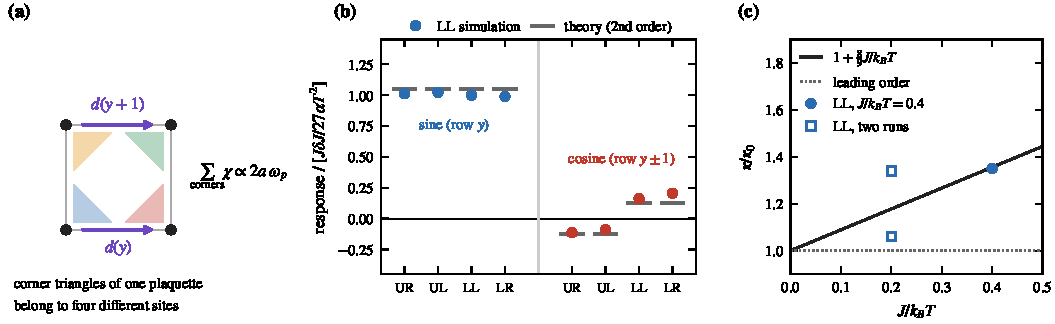
\includegraphics[width=\textwidth]{figs/highT.pdf}
\caption{High-temperature vorticity coupling. (a)~The four corner triangles of a plaquette belong to four different sites; their responses to the x-bond biases $d(y)$ and $d(y+1)$ add up to the lattice curl. (b)~Projections of the triangle responses onto the sine (row $y$) and cosine (rows $y\pm1$) of a sinusoidal shear, from stochastic LL simulations ($L=8$, 256 replicas, $\alpha=0.5$, $\kT=2.5J$) and the exact second-order kernel. (c)~Coupling constant $\kappa(T)/\kappa_0$ from the plaquette sum; the line is Eq.~\eqref{eq:kappaT}.}
\label{fig:highT}
\end{figure*}

\emph{Full-dynamics test of the selection rules.} Figure~\ref{fig:selection} shows LL simulations on a $32^2$ lattice. With a mirror present ($\theta=0,\pi/4$) the charge density vanishes at the $10^{-5}$ level even for strongly nonlinear drive, $\delta J=J$; the allowed $\sin4\theta$ term is below detection. In a strip with open edges the total charge follows the sign of the circulation, and its magnitude agrees with the second-order $\kappa(T)$; the leading order alone is off by $2.7\sigma$.

\begin{figure*}[t]
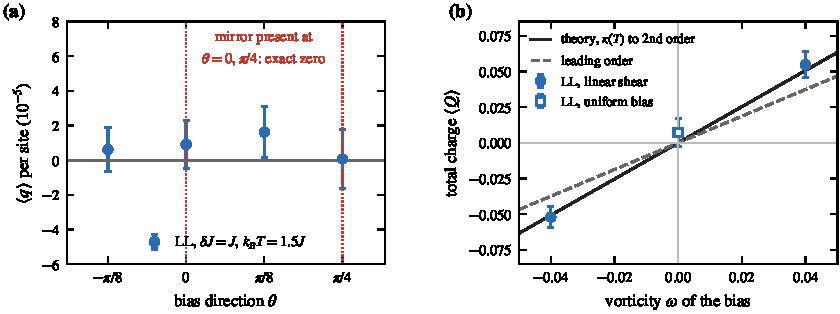
\includegraphics[width=0.95\textwidth]{figs/selection.pdf}
\caption{Selection rules in the full LL dynamics ($32^2$ lattice, 16 replicas, $\alpha=0.5$). (a)~Charge density for a uniform bias $\delta J=J$ at direction $\theta$ ($\kT=1.5J$). (b)~Total charge in a strip open in $y$ for a linear shear of vorticity $\pm\omega$ and for a uniform bias ($\kT=2.5J$). Lines: Eq.~\eqref{eq:kappa0} with $\kappa_0$ (dashed) and with $\kappa(T)$ of Eq.~\eqref{eq:kappaT} (solid).}
\label{fig:selection}
\end{figure*}

\emph{Spin--orbit coupling: an out-of-plane pseudo-field.} With interfacial DMI, $\mathbf D_{ij}=D(\hat z\times\hat e_{ij})$, and an out-of-plane FL bias $\vh^N_i=\delta D_z\,\hat z\times\sum_j\vS_j$, the pump $\dot E_N$ is no longer an eigenfunction of $\Delta$. We invert $\Delta$ by decomposing each single-spin monomial into spherical harmonics (Appendix~\ref{app:moments}) and find, per site,
\begin{equation}
\avg{q}=\frac{11}{5832\pi}\,\frac{\delta D_z\,D^2}{\alpha(\kT)^3},\qquad \avg{q}_{\rm eq}=-\frac{B_zD^2}{81\pi(\kT)^3},
\label{eq:soc}
\end{equation}
where the second expression is the equilibrium response to a Zeeman field on the same lattice. Comparing the two,
\begin{equation}
\Beff=-\frac{11}{72}\,\frac{\delta D_z}{\alpha}.
\label{eq:Beff}
\end{equation}
The out-of-plane bias acts on the topological charge as a magnetic field whose strength grows as $1/\alpha$. The $1/\alpha$ marks a dynamical pseudo-field rather than a true field, and it offers a way to separate the effect from Oersted and stray fields.

%=====================================================================
\section{Low temperature: the stream-function Boltzmann law}\label{sec:lowT}
%=====================================================================

\subsection{The skyrmion Hall drift as a gradient flow}

For well-formed skyrmions we work with Eq.~\eqref{eq:thiele}. We take the drift divergence-free, $\nabla\cdot\vueff=0$, and $\beta/\alpha$ uniform, and introduce the stream function $\psi_e$ through
\begin{equation}
\hat z\times\vueff=\nabla\psi_e,\qquad \nabla^2\psi_e=-\omega_e .
\label{eq:psi}
\end{equation}
Solving Eq.~\eqref{eq:thiele} for $\mathbf F=0$ and splitting the velocity by parity in $G$ gives
\begin{equation}
\vv=\underbrace{\frac{\beta}{\alpha}\vu-\frac{G^2\,\vueff}{\alpha^2\mathcal D^2+G^2}}_{\text{even in }G}\;\underbrace{-\,\mu\,\nabla(G\psi_e)}_{\text{odd in }G},
\label{eq:vsplit}
\end{equation}
with $\mu=\alpha\mathcal D/(\alpha^2\mathcal D^2+G^2)$.
The charge-odd, oblique part of the motion---the skyrmion Hall drift~\cite{Jiang2017,Litzius2017}---is exactly a gradient flow in the potential $G\psi_e$, with the same mobility $\mu$ that sets the diffusion constant $\mu\kT$. The charge-even part advects along level lines of $\psi_e$ and preserves any function of $\psi_e$. Hence, for a single skyrmion of charge $Q$,
\begin{equation}
P_Q(\vr)\propto\exp\big[-G_Q\,\psi_e(\vr)/\kT\big],\qquad G_Q=4\pi Qs,
\label{eq:boltzmann}
\end{equation}
independent of $\mathcal D$, $\alpha$ and the skyrmion shape.

This result separates kinetics from statistics. The Hall angle, $\tan\theta_H\sim G/(\alpha\mathcal D)$, depends on dissipation, and the Hall speed $\mu G\ueff$ is even nonmonotonic in $G$. The stationary statistics depend only on $G\ueff/\kT$. In a strip with uniform drift, skyrmions accumulate at one edge over a length $\ell_u=\kT/(G\ueff)$, and opposite charges go to opposite edges.

Figure~\ref{fig:stream} tests Eq.~\eqref{eq:boltzmann} with Thiele particle simulations in which the current $\vu$ enters directly and the prediction uses only $\psi_e$. In a cellular flow the slope of $\ln P_Q$ against $\psi_e$ is $0.987$--$0.995$ of $G/\kT$ for four combinations of $(\alpha,\beta)$, including one in which $\vu$ points against $\vueff$. In a strip the edge length agrees with $\ell_u$ to within 1\%.

\begin{figure*}[t]
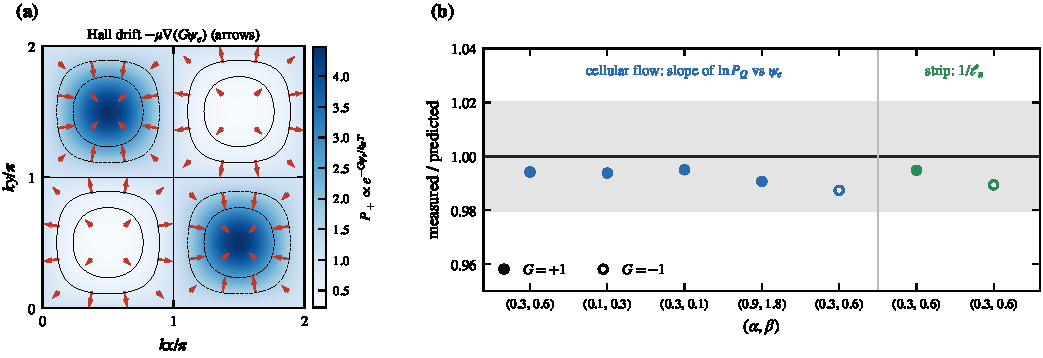
\includegraphics[width=\textwidth]{figs/stream.pdf}
\caption{Stream-function Boltzmann law. (a)~Stationary density of a $Q>0$ skyrmion in the cellular flow $\psi_e=1.5\sin kx\sin ky$ ($G/\kT=1$); contours are level lines of $\psi_e$ and arrows the Hall drift $-\mu\nabla(G\psi_e)$, which points toward the density maxima. (b)~Thiele particle simulations: slope of $\ln P_Q$ against $\psi_e$ in the cellular flow and inverse edge-accumulation length in a strip, divided by the predictions $G/\kT$ and $1/\ell_u$. Filled and open symbols are $G=+1$ and $-1$; the shaded band is $\pm2\%$.}
\label{fig:stream}
\end{figure*}

\subsection{Charge balance and segregation}

Transport cannot change the total charge; $Q$ changes only through lattice-scale nucleation and collapse of single skyrmions. Let $n_\pm$ be the densities, $s=n_++n_-$ and $\rho=n_+-n_-$. Pair creation and annihilation change $n_+$ and $n_-$ equally and drop out of the charge equation exactly:
\begin{equation}
\partial_t\rho=D_s\nabla^2\rho+\mu G\,\nabla\!\cdot\!(s\nabla\psi_e)+\mathcal B(\vr)-\nu\rho .
\label{eq:rate}
\end{equation}
Here $D_s=\mu\kT$, $\mathcal B=\Gamma_+-\Gamma_-$ is the nucleation bias and $\nu$ the collapse rate. By Theorem~2, $\mathcal B$ is a pseudoscalar odd in precession, so to linear order $\mathcal B\propto\omega$. Three results follow. In a closed sample $Q=\int\mathcal B\,\dd^2r/\nu\propto\oint\hat{\vv}\cdot\dd\mathbf l$: transport redistributes charge but does not create it. With open edges the Hall flux removes opposite charges through opposite edges. In linear response the charge density obeys
\begin{equation}
\rho^{\rm tr}_{\mathbf k}=-\frac{Gs}{\kT}\,\frac{k^2}{k^2+\ell_\nu^{-2}}\,\psi_{\mathbf k},\qquad \ell_\nu=\sqrt{D_s/\nu},
\label{eq:crossover}
\end{equation}
so the charge follows the potential $\psi_e$ for $k\ell_\nu\gg1$ and the vorticity for $k\ell_\nu\ll1$. The length $\ell_\nu$ interpolates between the low- and high-temperature forms of the topological response.

Without single events and with uniform pair creation, the mean-field equations have an exact stationary solution for any transport speed:
\begin{equation}
n_\pm=n_0\,e^{\mp G\psi_e/\kT},\quad n_+n_-=n_0^2,\quad \frac{\bar n}{n_0}=\big\langle e^{-G\psi_e/\kT}\big\rangle\ge1 .
\label{eq:segregation}
\end{equation}
A vortical flow therefore raises the total skyrmion number without creating net charge, while the product $n_+n_-$ stays uniform [Fig.~\ref{fig:segregation}(a)]. A many-body particle gas with pair creation and annihilation confirms both the density increase and the crossover length [Figs.~\ref{fig:segregation}(b) and (c)]. At $b=G\psi_{\max}/\kT=3$ the minority species in each cell drops to a few particles and mean-field theory overestimates the density by 8\%.

\begin{figure*}[t]
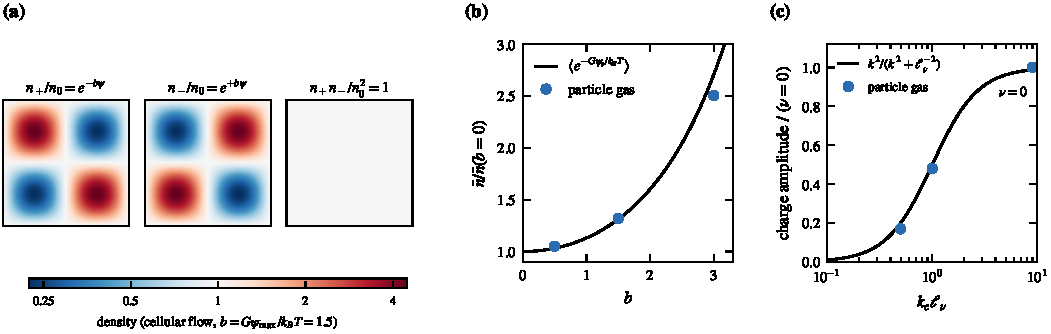
\includegraphics[width=\textwidth]{figs/segregation.pdf}
\caption{Charge segregation in a vortical flow. (a)~Mean-field densities of Eq.~\eqref{eq:segregation} in a cellular flow ($b=1.5$, logarithmic colour scale): the two species separate, but their product is uniform. (b)~Total density relative to $b=0$ from a many-body particle gas, against $\langle e^{-G\psi_e/\kT}\rangle$. (c)~Charge amplitude with single-skyrmion decay, relative to $\nu=0$, against $k_c\ell_\nu$; the line is the kernel of Eq.~\eqref{eq:crossover}.}
\label{fig:segregation}
\end{figure*}

%=====================================================================
\section{Thermal skyrmion--antiskyrmion pairs}\label{sec:pairs}
%=====================================================================

\subsection{Which pairs are driven apart}

For two objects with gyrocouplings $G_1,G_2$ and equal dissipation, eliminating the center of mass removes the charge-even advection. For $G_1=-G_2=G$ the relative coordinate $\vr=\vr_+-\vr_-$ obeys
\begin{equation}
\dot\vr=-2\mu\nabla_{\vr}\big[U(r)+G\,(\hat z\times\vueff)\cdot\vr\big]+\bm\eta,\qquad D_r=2\mu\kT .
\label{eq:pair}
\end{equation}
The relative drift $\vv_{\rm rel}=-2\mu G\,\hat z\times\vueff$ is perpendicular to the current. In general the relative drive is proportional to $G_1-G_2$: composites of equal charge travel together, and only charge-neutral pairs are pulled apart. The easy-plane vortex problem~\cite{Companion} is the special case $Q=pw/2$, where only vortex--antivortex pairs of equal core polarity are driven apart.

\subsection{Escape without binding}

In the Heisenberg model the skyrmion--antiskyrmion interaction is short ranged, without the logarithm that binds vortices~\cite{KosterlitzThouless1973,HalperinNelson1979}. Dissociation is therefore not activated, and the only length is the ratio of diffusion to drift,
\begin{equation}
\ell_u=\frac{D_r}{v_{\rm rel}}=\frac{\kT}{G|\ueff|},
\label{eq:ellu}
\end{equation}
in which both $\alpha$ and $\mathcal D$ cancel. Writing the hitting probability as $h=e^{-x/2\ell_u}g$ turns the drift--diffusion problem into a modified Helmholtz equation (Appendix~\ref{app:pair}). For a pair born at separation $R_0$ with an absorbing core of radius $a$,
\begin{equation}
P_{\rm esc}=1-\frac{I_0(R_0/2\ell_u)K_0(R_0/2\ell_u)}{K_0(a/2\ell_u)}\simeq\frac{\ln(R_0/a)}{\ln(4\ell_u/a)-\gamma_E}.
\label{eq:Pesc}
\end{equation}
The constant $\ln4-\gamma_E\approx0.81$ is not negligible: dropping it overestimates $P_{\rm esc}$ by 10--37\% over the range tested [Fig.~\ref{fig:escape}(a)]. The rate constant for non-geminate annihilation contains the same $K_0(a/2\ell_u)$, $k=2\pi D_r/[\ln(4\ell_u/a)-\gamma_E]$. In the steady state of pair creation at rate $\Gamma$ per area the denominators cancel:
\begin{equation}
n_f^2=\frac{\Gamma P_{\rm esc}}{k}=\frac{\Gamma\ln(R_0/a)}{2\pi D_r}.
\label{eq:nf}
\end{equation}
The free density does not depend on the drive. In a many-body gas with about one hundred particles of each sign, $n_f/n_{\rm pred}=0.97$--$1.04$ for $\ell_u/a$ from 5 to $\infty$, while $P_{\rm esc}$ changes by a factor of 2.2 [Fig.~\ref{fig:escape}(b)]. Table~\ref{tab:contrast} contrasts the result with the vortex case.

\begin{figure*}[t]
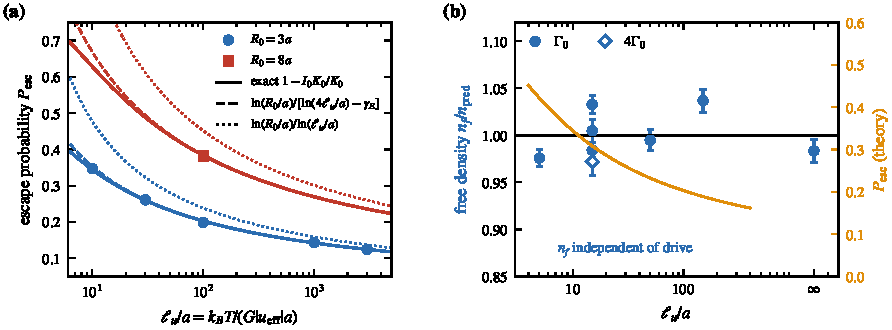
\includegraphics[width=0.95\textwidth]{figs/escape.pdf}
\caption{Pair escape and free density. (a)~Escape probability from two-particle Thiele simulations against the exact $K_0$ expression (solid), the asymptotic form of Eq.~\eqref{eq:Pesc} (dashed) and the form without the constant $\ln4-\gamma_E$ (dotted). (b)~Free density of a many-body gas relative to Eq.~\eqref{eq:nf} at creation rates $\Gamma_0$ and $4\Gamma_0$ (left axis), with the escape probability over the same range (right axis).}
\label{fig:escape}
\end{figure*}

\begin{table}[b]
\caption{Driven pairs of XY vortices and Heisenberg skyrmions.}
\label{tab:contrast}
\begin{ruledtabular}
\footnotesize
\begin{tabular}{lll}
 & XY vortices & Heisenberg skyrmions\\
\hline
Binding & $2\pi K\ln r$ & short ranged\\
Driven pairs & equal core polarity & all neutral pairs\\
Length & $r^*=2\pi K/(G\ueff)$ & $\ell_u=\kT/(G\ueff)$\\
Free density & $\propto|G\ueff|^{\pi K/\kT}$ & independent of $\ueff$\\
Drive visible in & density & correlation, edges\\
\end{tabular}
\end{ruledtabular}
\end{table}

\subsection{Pair correlation: the upstream shadow}

If the drive does not change the free density, where does it show up? In a dilute gas the pair density of the relative coordinate solves the same drift--diffusion problem with a ring source at $R_0$ and an absorbing core. Imposing absorption in every angular harmonic gives the exact two-body solution (Appendix~\ref{app:pair}). Two wakes compete. Geminate pairs are pushed downstream and form an excess wake, while the absorbing core casts a depleted wake of the same form, $e^{\rho\cos\theta}K_0(\rho)$ with $\rho=r/2\ell_u$ [Fig.~\ref{fig:paircorr}(a)]. With the density fixed by flux balance, the two wakes cancel at large distance to leading order---the same identity that makes $n_f$ drive independent. What survives is the shadow near the core, so the dipole component $g_1$ of the pair correlation is negative everywhere. Pairs sit preferentially \emph{upstream} of the Hall separation, opposite to the naive expectation from stretched geminate pairs. The many-body simulations confirm the exact solution in detail [Figs.~\ref{fig:paircorr}(b) and (c)]. The peak of $|g_1|$ is 0.02, 0.13 and 0.17 for $R_0/\ell_u=0.2$, 1 and 2, so the asymmetry is observable for $R_0\gtrsim\ell_u$.

\begin{figure*}[t]
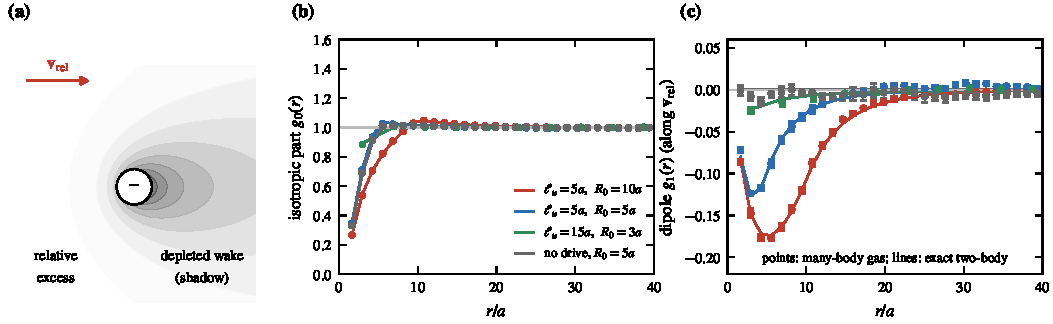
\includegraphics[width=\textwidth]{figs/paircorr.pdf}
\caption{Upstream shadow in the pair correlation. (a)~Schematic of the depleted wake $e^{\rho\cos\theta}K_0(\rho)$ cast by the absorbing core in the frame of the relative drift $\vv_{\rm rel}$. (b),(c)~Isotropic and dipole components of the skyrmion--antiskyrmion correlation from a many-body gas (points) and the exact two-body solution (lines).}
\label{fig:paircorr}
\end{figure*}

\emph{Magnitudes.} For a film with $M_s=1$~MA/m, thickness 1~nm, $\ueff\approx100$~m/s and room temperature, $G=4\pi M_st/\gamma$ gives $\ell_u\approx0.6$~nm. Real films are thus in the strongly driven regime $R_0\gtrsim\ell_u$, where the shadow is large. The thermal linear regime opens near $\beta\approx\alpha$ or at small currents. In either regime all effects of this section vanish at $\beta=\alpha$.

%=====================================================================
\section{Vorticity-driven nucleation: the rotational channel}\label{sec:nucleation}
%=====================================================================

\subsection{Two channels}

Theorem~2 guarantees the nucleation bias $\mathcal B\propto\omega$ but not its size. Before describing simulations, we show that the bias need not be proportional to $\ueff$. At $\beta=\alpha$ the current-driven equation is the equilibrium Landau--Lifshitz--Gilbert equation written with a convective derivative, $D_t\vS=-\vS\times\vh+\alpha\vS\times D_t\vS$ with $D_t=\partial_t+(\vu\cdot\nabla)$. For uniform $\vu$ this is a Galilean boost, and the stationary measure is Boltzmann. A shear flow is locally a strain plus a rigid rotation at angular velocity $\Omega=\omega/2$ [Fig.~\ref{fig:rotation}(a)]. The strain is a traceless symmetric tensor and cannot enter a scalar rate at linear order on a lattice with a fourfold axis, so only $\Omega$ matters. For a rotation,
\begin{equation}
(\vu\cdot\nabla)\vS=-\Omega\,\mathcal G\vS+\Omega\,\hat z\times\vS,\qquad \mathcal G\vS\equiv\hat z\times\vS-\partial_\varphi\vS,
\label{eq:Gdecomp}
\end{equation}
where $\mathcal G$ generates joint rotations of space and spin. Exchange, interfacial DMI, $B_z$ and uniaxial anisotropy are invariant under joint rotations, so the $\mathcal G$ term is removed by a change of frame. What remains rotates the spins alone. In LL form it is a precession field with no dissipative partner,
\begin{equation}
\dot\vS=-\vS\times(\vh-\Omega\hat z)-\alpha\,\vS\times(\vS\times\vh).
\label{eq:preconly}
\end{equation}
If $E$ were invariant under spin-only rotations about $\hat z$, a rotating spin frame would remove this term as well; the DMI locks the spin frame to the lattice and prevents that. The vorticity therefore biases nucleation through two channels,
\begin{equation}
\ln\Gamma_Q(\omega)=\ln\Gamma_Q(0)+c\,Q\,\omega,\qquad c=c_{\rm rot}+c_{\rm FL}\,\frac{\beta-\alpha}{\alpha}.
\label{eq:twochannel}
\end{equation}
The second term is the pseudo-energy channel of Secs.~\ref{sec:highT} and~\ref{sec:lowT}, carried by $\ueff$. The first is a spin--orbit effect of the rotation of the flow itself. It is reminiscent of the Barnett effect~\cite{Barnett1915}, in which mechanical rotation magnetizes a body, but here only the precessional half of the Barnett field appears.

\subsection{What a precession-only field does}

The effect of Eq.~\eqref{eq:preconly} depends on whether damping or precession is faster.

\emph{Strong damping} ($\alpha\kT\gg J$). The expansion of Sec.~\ref{sec:highT} with $\vh^N=-\Omega\hat z$ gives $\dot E_N=\Omega D\sum\hat e_{ij}\cdot(\vS_i\times\vS_j)$, a Bloch-type DMI density. The static and dissipative pieces cancel exactly and only the precessional piece survives:
\begin{equation}
\avg{q}_{\rm rot}=\frac{\Omega D^2}{324\pi\,\alpha^2(\kT)^3},\qquad \Beff=-\frac{\Omega}{4\alpha^2}.
\label{eq:rotstrong}
\end{equation}

\emph{Weak damping} ($\alpha\to0$). The precessional flow then conserves $E'=E+\Omega M$ with $M=\sum S^z$. Damping and noise become a slow diffusion between $E'$ shells, and the zero-flux condition is independent of $\alpha$. If the flow mixes each shell, the stationary measure is
\begin{equation}
p\propto\exp\!\Big[-\frac{E(1-\Omega r)+\Omega M}{\kT}\Big],\qquad r=\frac{\avg{\nabla M\cdot\nabla E}_E}{\avg{|\nabla E|^2}_E}.
\label{eq:rotweak}
\end{equation}
The precession-only field thus acts as a true Zeeman field $\Beff=-\Omega=-\omega/2$, with a small renormalization of the temperature; $r=0$ at $B=0$ by symmetry and $r\approx-1/(4J+B)$ in a saturated ferromagnet. Without DMI, $M$ is conserved as well, the reduction fails, and the effect vanishes exactly.

Figure~\ref{fig:rotation}(b) confirms both limits with LL simulations ($L=32$, $J=D=1$). For $\alpha\kT\lesssim0.2J$ the response equals the equilibrium response to a real field $B=-\Omega$ to within a few percent; at $\kT=4J$ it matches Eq.~\eqref{eq:rotstrong}. The response vanishes for $D=0$, is odd in $\Omega$, and adds to the response to a real field. The crossover sits at $\alpha\kT\approx J$. Typical skyrmion hosts at room temperature have $\alpha\sim0.01$--$0.3$ and $\kT\ll J$, deep in the weak-damping regime.

\begin{figure*}[t]
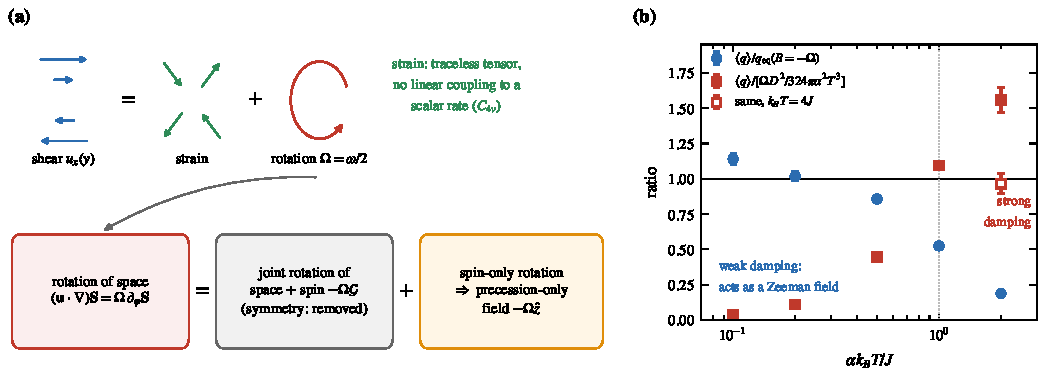
\includegraphics[width=\textwidth]{figs/rotation.pdf}
\caption{The rotational channel. (a)~A shear flow is a strain plus a rotation $\Omega=\omega/2$. Advection by the rotation equals a joint rotation of space and spin, which is a symmetry of the energy, plus a rotation of the spins alone, which acts as the precession-only field $-\Omega\hat z$ of Eq.~\eqref{eq:preconly}. (b)~Charge response to a uniform precession-only field from stochastic LL simulations ($L=32$, $J=D=1$, $\kT=2J$ unless noted), divided by the equilibrium response to a real field $B=-\Omega$ (circles) and by the strong-damping formula of Eq.~\eqref{eq:rotstrong} (squares).}
\label{fig:rotation}
\end{figure*}

\subsection{Simulations of a chiral ferromagnet}

We simulate the stochastic LLG equation with Zhang--Li torques on a $64^2$ lattice with $J=1$, interfacial DMI $D=0.3J$, field $B=0.12J$ and $\kT=0.5J$. The field selects $Q=-1$ skyrmions of radius $2.56a$, and undriven nucleation has an Arrhenius barrier of about $6J$. The drive is a sinusoidal shear $u_x(y)$ with maximal vorticity $0.0039$. Nucleation and collapse are counted by tracking objects that survive at least $\tau_c=10$, binned in $\omega(y)$, and the slope $s=\dd\ln\Gamma/\dd\omega$ gives $c=s/Q$.

\begin{figure*}[t]
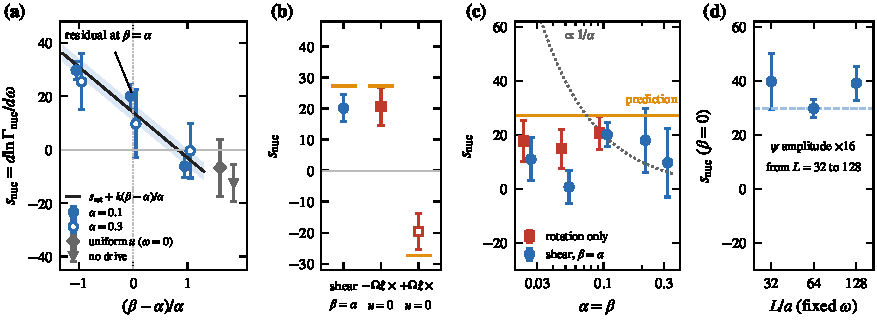
\includegraphics[width=\textwidth]{figs/nucleation.pdf}
\caption{Vorticity-biased nucleation in a chiral ferromagnet ($D=0.3J$, $B=0.12J$, $\kT=0.5J$, $L=64$). (a)~Nucleation slope against $(\beta-\alpha)/\alpha$ for two damping constants, with the two-channel fit of Eq.~\eqref{eq:twochannel} and the null controls. (b)~Shear at $\beta=\alpha$ compared with the rotation-only drive $D_t=\partial_t\pm(\omega/2)\hat z\times$ at $u=0$; orange bars are the weak-damping prediction $\pm27.3$. (c)~Damping dependence at $\beta=\alpha$; the dotted line shows the $1/\alpha$ scaling of the strong-damping limit, which is excluded. (d)~Size dependence at fixed vorticity.}
\label{fig:nucleation}
\end{figure*}

\emph{The bias and its residual.} The nucleation bias exists at $9\sigma$, is linear in the drive and vanishes for uniform current and for no drive [Fig.~\ref{fig:nucleation}(a)]. At fixed $(\beta-\alpha)/\alpha$ the two damping constants agree. But the bias does not vanish at $\beta=\alpha$: the data fit Eq.~\eqref{eq:twochannel} with $s_{\rm rot}=14\pm2$ and a pseudo-energy slope $-17\pm2.6$. This residual is the rotational channel.

\emph{Isolating the rotational channel.} Replacing the advection by the pure rotation $D_t=\partial_t+(\omega/2)\hat z\times$ at $\vu=0$ reproduces the residual of the $\beta=\alpha$ shear, including its sign [Fig.~\ref{fig:nucleation}(b)]. Reversing the rotation reverses the response: the odd part is $20.2\pm4.2$ ($4.8\sigma$) and the even part $0.5\pm4.2$. The rotation-only response is independent of damping between $\alpha=0.025$ and $0.1$ (mean $18.2\pm3.9$), ruling out the $1/\alpha$ growth of the strong-damping limit [Fig.~\ref{fig:nucleation}(c)]. A two-harmonic shear, in which $\omega$ and $\psi_e$ have different profiles, gives a stream-function coefficient consistent with zero at both $\beta=0$ and $\beta=\alpha$, and the slope does not change when the system size, and with it the amplitude of $\psi_e$, grows by a factor of four at fixed $\omega$ [Fig.~\ref{fig:nucleation}(d)]. The bias is a local response to vorticity.

\emph{Magnitude.} In the weak-damping regime, Eq.~\eqref{eq:rotweak} states that the rotational drive shifts the whole stationary measure to $(B-\Omega,\,T(1+\Omega r))$. The rate therefore shifts as the undriven rate does when the field and temperature are changed, prefactor included:
\begin{equation}
s_{\rm rot}=-\frac12\frac{\partial\ln\Gamma_0}{\partial B}+\frac{rT}{2}\frac{\partial\ln\Gamma_0}{\partial T}.
\label{eq:spred}
\end{equation}
Paired undriven runs at $B=0.11J$ and $0.13J$ give $\partial\ln\Gamma_0/\partial B=-57.5\pm2.3$, so $s_{\rm rot}=27.3\pm1.1$ with no adjustable parameter. The barrier slope alone would predict about 55, a factor of 2.7 too large, because the prefactor compensates much of the barrier change.

The same reasoning applies to the population. In a local steady state the density of established skyrmions is $n=\Gamma_{\rm nuc}/\nu$, so the population slope $s_{\rm nuc}-s_{\rm col}$ reflects the stationary measure alone. Figure~\ref{fig:magnitude}(a) compares measured and predicted slopes over a temperature range in which the predicted population slope falls by more than a factor of two, because the thermal magnetization deficit of a skyrmion shrinks [Fig.~\ref{fig:magnitude}(c)], and at three DMI strengths at fixed $B/D^2$. The measured slopes follow the predicted dependence with a constant ratio, $F_{\rm pop}=0.85\pm0.08$ (weighted mean over $\kT=0.45$--$0.60J$, $\chi^2=0.44$ for 3 degrees of freedom), and the population slope agrees with a direct count of skyrmion density [Fig.~\ref{fig:magnitude}(b)]. The weak-damping Zeeman equivalence thus captures the dependence of the rotational channel on damping, DMI and temperature, and its magnitude to $15\pm8\%$.

\begin{figure*}[t]
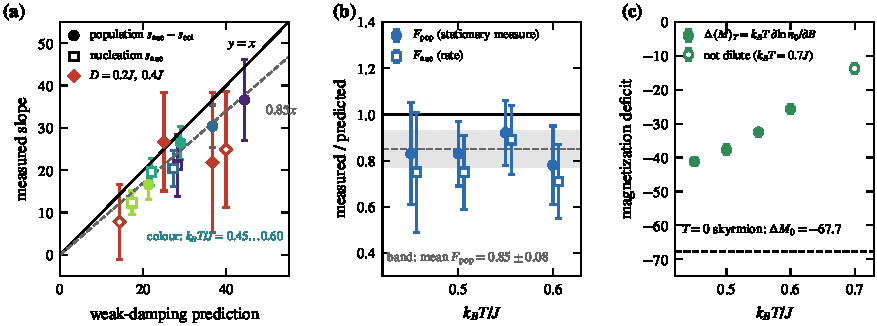
\includegraphics[width=\textwidth]{figs/magnitude.pdf}
\caption{Magnitude of the rotational channel. (a)~Measured against predicted slopes for the population $s_{\rm nuc}-s_{\rm col}$ (filled) and nucleation $s_{\rm nuc}$ (open), at $\kT/J=0.45$--$0.60$ (colour) and at $D=0.2J$, $0.4J$ with $B/D^2$ fixed (diamonds). Predictions use only undriven rates, Eq.~\eqref{eq:spred}. (b)~Ratio of measured to predicted slope; the band is the weighted mean $F_{\rm pop}=0.85\pm0.08$. (c)~Thermal magnetization deficit of a skyrmion, $\Delta\avg{M}_T=\kT\,\partial\ln n_0/\partial B$, compared with the relaxed $T=0$ skyrmion.}
\label{fig:magnitude}
\end{figure*}

Two alternative explanations of the remaining 15\% can be excluded. The temperature term of Eq.~\eqref{eq:spred} is only 0.6--5\% of the prediction, so an error in $r$ cannot account for it. If only the zero-temperature Zeeman energy of the skyrmion shifted, the ratio would be $|\Delta M_0|/|\Delta\avg{M}_T|\approx1.8$ rather than below one. The shortfall resides in the stationary measure, since $F_{\rm pop}$ agrees with the nucleation ratio and does not depend on the tracking time $\tau_c$. Incomplete mixing of the $E'$ shells at low temperature would make $F_{\rm pop}$ rise toward one with temperature; no rise is seen between $\kT=0.45J$ and $0.60J$, although the statistics cannot exclude a modest one. At $2\sigma$ from unity, the shortfall does not require a new mechanism, and we leave its origin open.

%=====================================================================
\section{Discussion}\label{sec:discussion}
%=====================================================================

\subsection{A hierarchy of mechanisms}

The results organize into three levels, each controlled by a different object. \emph{Symmetry} decides whether a net charge is allowed: out of equilibrium precession breaks time reversal, so only orientation-reversing operations matter. \emph{Sources} decide how much net charge appears: the local pseudo-energy coupling $-\kappa\int\omega q$ at high temperature, and the nucleation bias at low temperature, which itself has a pseudo-energy part $\propto\ueff$ and a rotational part. \emph{Transport}---the skyrmion Hall drift---decides where the charge goes. It separates and redistributes charge but cannot create it in a closed sample, it acts only through $G\ueff/\kT$, and it changes the total density only if the flow has vorticity. The kernel of Eq.~\eqref{eq:crossover} links the last two levels through the length $\ell_\nu$.

\subsection{Why the simple model is a reliable guide}

Each result rests on a structural feature of the equations of motion rather than on details of the model. The selection rules use only Theorem~1, that is, the fact that precession contains one cross product and damping two. They therefore hold for any energy, any lattice and both torque channels. The low-temperature results use only the structure of the Thiele equation---a gyrocoupling odd in $Q$ and a symmetric dissipation---and $\nabla\cdot\vueff=0$; they are independent of skyrmion size and profile. This is why the stationary distribution, escape probability and free density were unchanged when $\alpha$ varied by a factor of 18 in our simulations. The rotational channel uses only the joint rotation symmetry of exchange, interfacial DMI and the Zeeman energy, which holds in every isotropic thin film with $C_{\infty v}$ symmetry, and the weak-damping condition $\alpha\kT\ll J$, which real skyrmion hosts satisfy by a wide margin. The quantitative prediction, Eq.~\eqref{eq:spred}, requires no microscopic input beyond the measured field and temperature dependence of the undriven nucleation rate, which is directly accessible in experiment.

\subsection{Experimental consequences}

\emph{Null test at $\beta=\alpha$.} Edge accumulation, pair statistics and the pseudo-energy part of the nucleation bias vanish when $\ueff=0$. Tuning $\beta/\alpha$ by composition or temperature while monitoring them measures $\beta$ independently of other methods.

\emph{Net charge from circulation.} Ohmic currents in a uniform film are curl free. Vorticity of $\vu$ or $\vueff$ therefore requires a spatial variation of the conductivity, the spin polarization or $\beta/\alpha$, for example across the interface of a lateral heterostructure or along a thickness or composition gradient. The predicted net charge is proportional to the circulation and absent in a uniform film. Edge accumulation under uniform current is charge separation, not creation, and the two are distinguished by counting both edges.

\emph{Current rotation as a magnetic field.} The rotational channel predicts that a sheared current biases skyrmion nucleation as a local magnetic field $\Beff=-\omega/2$ (in units where $\gamma=1$; $\Beff=-\hbar\omega/(2g\mu_B)$ in physical units for the spin-velocity vorticity $\omega$), even when $\beta=\alpha$. The sign follows the circulation of the current, and the magnitude follows from the measured field sensitivity of the undriven nucleation rate. Where the spin-current density varies across the film, for example at the boundary between regions of different spin polarization, this provides a field-free and locally controllable way to bias skyrmions of one sign.

\emph{Field-free charge from unconventional spin--orbit torque.} An out-of-plane spin polarization, available in low-symmetry crystals, combined with interfacial DMI acts as $\Beff\propto-\delta D_z/\alpha$; the $\alpha$ dependence separates it from Oersted fields. In films whose DMI pattern lacks mirrors, the skyrmion balance under uniform current depends on current direction as $\sin2\theta$ ($D_2$) or $\sin4\theta$ ($D_4$).

\emph{Pair statistics.} In strongly driven films, skyrmion--antiskyrmion correlations are biased upstream of the Hall separation, while the density of free skyrmions is unchanged by the current. Time-resolved imaging of thermally activated textures~\cite{Zazvorka2019} can test both statements.

\subsection{Outlook}

Antiferromagnetic skyrmions have $G=0$. They should show neither Hall-driven segregation nor pair splitting, yet the high-temperature vorticity coupling and the rotational channel, which do not rely on $G$, remain. They therefore offer a sharp test of the separation between sources and transport. Extensions to three-dimensional textures, where the analog of $G$ is a tensor, are left for future work.

%=====================================================================
\section{Conclusion}\label{sec:conclusion}
%=====================================================================

Nonreciprocal spin couplings change the rules that decide whether a magnet carries net topological charge. Because precession, unlike damping, is odd under improper spin rotations, it supplies the time-reversal breaking of a magnetic field once the magnet is out of equilibrium, and only the orientation-reversing operations of the plane remain to be broken. Uniform currents therefore cannot create net charge in a mirror-symmetric film; vorticity can. At low temperature the skyrmion Hall drift turns out to be an exact gradient flow, which yields a Boltzmann law for skyrmion positions, a drive-independent density of free skyrmions and an upstream shadow in their pair correlation. Finally, the local rotation of a sheared current acts on the spins as a precession-only field that, in the weak-damping regime of real materials, is equivalent to a Zeeman field $-\omega/2$. This rotational channel survives at $\beta=\alpha$, where every effect carried by the effective drift disappears, and its dependence on temperature, damping and DMI follows from undriven nucleation rates alone. Current vorticity thus emerges as a control parameter for topological charge in its own right.

\begin{acknowledgments}
Large-scale nucleation simulations were carried out with the assistance of an AI coding agent; all analytic results were checked independently by exact series evaluation and stochastic simulations.
\end{acknowledgments}

\appendix

\section{Pseudo-energy equation}\label{app:pseudo}

Let $b=b_{\rm prec}+b_{\rm diss}+b_N$ be the drift of Eq.~\eqref{eq:LL}, with $b_{\rm prec}=-c_p\vS\times\vh$ divergence free and energy conserving, $b_{\rm diss}=-\alpha\nabla E$, and $b_N$ the nonreciprocal drift, which is divergence free on $(S^2)^N$~\cite{Companion}. Let $\mathcal L$ be the Fokker--Planck operator. For $p=p_0(1+\phi)$, $\mathcal Lp_0=\beta_Tp_0\dot E_N$ and $\mathcal L(p_0\phi)=p_0[\alpha\kT\Delta\phi-\alpha\nabla E\cdot\nabla\phi-b_{\rm prec}\cdot\nabla\phi]$. Stationarity at first order gives $\tilde L\phi=-\beta_T\dot E_N$; setting $\phi=-\beta_TE_1$ yields Eq.~\eqref{eq:pseudo}.

\section{Exact high-temperature moments}\label{app:moments}

We expand $E_1=(\alpha\kT\Delta)^{-1}\dot E_N-(\alpha\kT\Delta)^{-1}L_1(\alpha\kT\Delta)^{-1}\dot E_N+\dots$, with $L_1=-\alpha\nabla E\cdot\nabla+(\vS\times\vh)\cdot\nabla$, and $p_0$ to first order in $E/\kT$:
\begin{equation}
\avg{\chi}=-\beta_T\Big[\avg{\chi E_1^{(1)}}_0-\beta_T\avg{\chi E_1^{(1)}E}_0+\frac{\avg{\chi L_1E_1^{(1)}}_0}{6\alpha\kT}\Big].
\end{equation}
Because $\Delta\chi=-6\chi$ and $\Delta$ is self-adjoint, no inverse is needed for the $\delta J$ kernel. All averages are polynomial moments over independent uniform unit vectors,
\begin{equation}
\avg{x^{2p}y^{2q}z^{2r}}=\frac{(2p-1)!!\,(2q-1)!!\,(2r-1)!!}{(2p+2q+2r+1)!!}.
\end{equation}
In units of $J\delta J/27\alpha\kT^2$, with $d(y)$ the bias of the $x$ bonds in row $y$, the corner response is $\chi_{\rm UR}(y)=[1+\tfrac49J/\kT]\,d(y)-\tfrac49(J/\kT)\,d(y+1)$; the plaquette sum is $2(1+\tfrac89J/\kT)\,\omega_p$. For the spin--orbit and rotational cases $\dot E_N$ contains non-eigenfunctions. We invert $\Delta$ by decomposing each single-spin monomial into spherical harmonics with the projection $H(p)=\sum_k(-1)^k\frac{(2n-2k-1)!!}{(2n-1)!!\,2^kk!}\,r^{2k}\Delta^kp$ and dividing each product of harmonics by $-\sum_il_i(l_i+1)$. A cluster of $8\times8$ sites suffices; the results are converged at the smallest cluster radius tested.

\section{Drift--diffusion with an absorbing disk}\label{app:pair}

With relative drift $v_{\rm rel}=D_r/\ell_u$ along $\hat x$, the substitution $c=e^{x/2\ell_u}\varphi$ gives $(\nabla^2-1/4\ell_u^2)\varphi={\rm source}$. The hitting probability from $\vr_0$ is $h\approx e^{-x_0/2\ell_u}K_0(r_0/2\ell_u)/K_0(a/2\ell_u)$ to leading order in $a/\ell_u$, and averaging over the angle of birth gives Eq.~\eqref{eq:Pesc}. A uniform density at infinity flowing onto the core gives a flux $2\pi D_rn^2/K_0(a/2\ell_u)$. For the pair correlation with a ring source we use Graf's addition theorem and impose absorption in every harmonic $m$. Writing $z_0=R_0/2\ell_u$, $z_a=a/2\ell_u$ and $\gamma_m=(\Gamma/2\pi D_r)I_m(z_0)K_m(z_0)$, the condition $\varphi(z_a,\theta)=0$ fixes the coefficients $B_m=-\epsilon_m(-1)^mI_m(z_a)(n^2+\gamma_m)/K_m(z_a)$, and flux balance, evaluated with the Wronskian $I_mK_m'-I_m'K_m=-1/\rho$, fixes $n^2$. Treating the core as a monopole only would leave an $O(a/\ell_u)$ dipole error comparable to the signal, so the full harmonic treatment is required.

\section{Numerical methods}\label{app:numerics}

\emph{Stochastic LL and LLG.} Stratonovich Heun integration with renormalization of $|\vS|$ after predictor and corrector, $\dd t=\min(0.01,0.005/\alpha\kT)$ for the high-temperature runs and $\dd t=0.02$ (checked against $0.01$) for the chiral ferromagnet. Errors are block errors or replica$\times$time-block jackknife errors.

\emph{Nucleation counting.} Topological objects are tracked through the Berg--L\"uscher density; a nucleation (collapse) is the birth (death) of a tracked $Q=-1$ object that lives at least $\tau_c$. Rates are binned in 16 bands of $\omega(y)$ and slopes are obtained by Poisson regression. Results at $\tau_c=5$ and 20 lead to the same conclusions.

\emph{Thiele particles and many-body gas.} Euler--Maruyama integration of the full equation of motion of each object in the laboratory frame. Pair escape uses adaptive steps $\dd t\propto(r-a)^2/D_r$ near the core. The many-body gas uses $\dd t=0.1$ with a Brownian-bridge crossing probability $\exp[-(d_0-a)(d_1-a)/(D_r\dd t)]$ for annihilation and Poisson pair creation.

\emph{Code and data.} All scripts and data are available in the accompanying repository.

\begin{thebibliography}{99}

\bibitem{BelavinPolyakov1975} A. A. Belavin and A. M. Polyakov, Metastable states of two-dimensional isotropic ferromagnets, JETP Lett. \textbf{22}, 245 (1975).

\bibitem{Muhlbauer2009} S. M\"uhlbauer, B. Binz, F. Jonietz, C. Pfleiderer, A. Rosch, A. Neubauer, R. Georgii, and P. B\"oni, Skyrmion lattice in a chiral magnet, Science \textbf{323}, 915 (2009).

\bibitem{NagaosaTokura2013} N. Nagaosa and Y. Tokura, Topological properties and dynamics of magnetic skyrmions, Nat. Nanotechnol. \textbf{8}, 899 (2013).

\bibitem{Fert2017} A. Fert, N. Reyren, and V. Cros, Magnetic skyrmions: advances in physics and potential applications, Nat. Rev. Mater. \textbf{2}, 17031 (2017).

\bibitem{ZhangLi2004} S. Zhang and Z. Li, Roles of nonequilibrium conduction electrons on the magnetization dynamics of ferromagnets, Phys. Rev. Lett. \textbf{93}, 127204 (2004).

\bibitem{Thiaville2005} A. Thiaville, Y. Nakatani, J. Miltat, and Y. Suzuki, Micromagnetic understanding of current-driven domain wall motion in patterned nanowires, Europhys. Lett. \textbf{69}, 990 (2005).

\bibitem{Fruchart2021} M. Fruchart, R. Hanai, P. B. Littlewood, and V. Vitelli, Non-reciprocal phase transitions, Nature \textbf{592}, 363 (2021).

\bibitem{Hanai2024} R. Hanai, Nonreciprocal frustration: time crystalline order-by-disorder phenomenon and a spin-glass-like state, Phys. Rev. X \textbf{14}, 011029 (2024).

\bibitem{Das2002} J. Das, M. Rao, and S. Ramaswamy, Nonequilibrium steady states of the isotropic classical magnet, Europhys. Lett. \textbf{60}, 418 (2002).

\bibitem{Companion} C. Won, Nonreciprocal spin couplings: measure preservation, pseudo-energies and no-go theorems (in preparation).

\bibitem{Thiele1973} A. A. Thiele, Steady-state motion of magnetic domains, Phys. Rev. Lett. \textbf{30}, 230 (1973).

\bibitem{BergLuscher1981} B. Berg and M. L\"uscher, Definition and statistical distributions of a topological number in the lattice O(3) $\sigma$-model, Nucl. Phys. B \textbf{190}, 412 (1981).

\bibitem{Jiang2017} W. Jiang, X. Zhang, G. Yu, W. Zhang, X. Wang, M. B. Jungfleisch, J. E. Pearson, X. Cheng, O. Heinonen, K. L. Wang, Y. Zhou, A. Hoffmann, and S. G. E. te Velthuis, Direct observation of the skyrmion Hall effect, Nat. Phys. \textbf{13}, 162 (2017).

\bibitem{Litzius2017} K. Litzius \emph{et al.}, Skyrmion Hall effect revealed by direct time-resolved X-ray microscopy, Nat. Phys. \textbf{13}, 170 (2017).

\bibitem{KosterlitzThouless1973} J. M. Kosterlitz and D. J. Thouless, Ordering, metastability and phase transitions in two-dimensional systems, J. Phys. C \textbf{6}, 1181 (1973).

\bibitem{HalperinNelson1979} B. I. Halperin and D. R. Nelson, Resistive transition in superconducting films, J. Low Temp. Phys. \textbf{36}, 599 (1979).

\bibitem{Barnett1915} S. J. Barnett, Magnetization by rotation, Phys. Rev. \textbf{6}, 239 (1915).

\bibitem{Zazvorka2019} J. Z\'azvorka \emph{et al.}, Thermal skyrmion diffusion used in a reshuffler device, Nat. Nanotechnol. \textbf{14}, 658 (2019).

\end{thebibliography}

\end{document}
